\documentclass[12pt,a4paper]{report}

%adjust your page margins here
\usepackage[top=0.70in, bottom=0.70in, left=0.8in,right=0.80in]{geometry} % setting the page alignment with this package
\usepackage[pdftex]{graphicx} %for embedding images
\usepackage[ bookmarks,  colorlinks=false]{hyperref} %for creating links in the pdf version and other additional pdf attributes, no effect on the printed document
\hypersetup{%
    pdfborder = {0 0 0}
}
\usepackage[final]{pdfpages} %for embedding another pdf, remove if not required
\usepackage{float} %used for figure placement with H as a parameter
\usepackage{hyperref}
\usepackage{pslatex} % for times new roman, old package, but works
\usepackage{array} % for making text bold in table
\usepackage{setspace}
\usepackage{float}
\usepackage{enumerate}
\usepackage{longtable}

\usepackage[font=small,labelfont=bf]{caption}
\def\figurename{\textbf{Figure }}

\usepackage{listings}
\usepackage{color}

\definecolor{dkgreen}{rgb}{0,0.6,0}
\definecolor{gray}{rgb}{0.5,0.5,0.5}
\definecolor{mauve}{rgb}{0.58,0,0.82}
 
\lstset{ %
  language=Java,                % the language of the code
  basicstyle=\footnotesize,           % the size of the fonts that are used for the code
  numbers=left,                   % where to put the line-numbers
  numberstyle=\tiny\color{gray},  % the style that is used for the line-numbers
  stepnumber=1,                   % each line is numbered
  numbersep=5pt,                  % how far the line-numbers are from the code
  backgroundcolor=\color{white},      % choose the background color. You must add \usepackage{color}
  showspaces=false,               % show spaces adding particular underscores
  showstringspaces=false,         % underline spaces within strings
  showtabs=false,                 % show tabs within strings adding particular underscores
  frame=single,                   % adds a frame around the code
  rulecolor=\color{black},        % if not set, the frame-color may be changed on line-breaks within not-black text (e.g. commens (green here))
  tabsize=2,                      % sets default tabsize to 2 spaces
  captionpos=b,                   % sets the caption-position to bottom
  breaklines=true,                % sets automatic line breaking
  breakatwhitespace=false,        % sets if automatic breaks should only happen at whitespace
  title=\lstname,                   % show the filename of files included with \lstinputlisting;
                                  % also try caption instead of title
  keywordstyle=\color{blue},          % keyword style
  commentstyle=\color{dkgreen},       % comment style
  stringstyle=\color{mauve},         % string literal style
  escapeinside={\%*}{*)},            % if you want to add a comment within your code
  morekeywords={*,...}               % if you want to add more keywords to the set
}

%For the header and footer
\usepackage{fancyhdr}
\fancypagestyle{plain}{%
\fancyfoot[L]{\emph{Master Informatic, Unicersity Bordeaux 1}} % except the center
\fancyfoot[R]{\thepage}
\renewcommand{\headrulewidth}{0.4pt}
\renewcommand{\footrulewidth}{0.4pt}
}

\pagestyle{fancy}

\rhead{\emph{TRAVEL RESERVATION SERVICE}}

\fancyfoot[LO,LE]{\emph{Master Informatic, Unicersity Bordeaux 1}}
\cfoot{}
\fancyfoot[RO, RE]{\thepage}
\renewcommand{\headrulewidth}{0.4pt}
\renewcommand{\footrulewidth}{0.4pt}
%For the header and footer Over

%Page Border
\usepackage{pgf}
\usepackage{pgfpages}

\pgfpagesdeclarelayout{boxed}
{
  \edef\pgfpageoptionborder{0pt}
}
{
  \pgfpagesphysicalpageoptions
  {%
    logical pages=1,%
  }
  \pgfpageslogicalpageoptions{1}
  {
    border code=\pgfsetlinewidth{2pt}\pgfstroke,%
    border shrink=\pgfpageoptionborder,%
    resized width=.95\pgfphysicalwidth,%
    resized height=.95\pgfphysicalheight,%
    center=\pgfpoint{.5\pgfphysicalwidth}{.5\pgfphysicalheight}%
  }%
}
\pgfpagesuselayout{boxed}
\setlength{\parindent}{1cm}
%GLOBAL SETTINGS OVER, DOCUMENT BEGINS
\begin{document}
\renewcommand\bibname{References}
\lhead{ }

%FROM HERE YOUR PAGES START GETTING ADDED

% includes the cover page
\newpage
\begin{center}
\thispagestyle{empty}
\Large{\textbf{A PROJECT REPORT\\ \large{ON}}}\\[0.7cm]
\LARGE{\textsc {\textbf{TRAVEL RESERVATION SERVICE}}}\\[0.5cm]
\vspace{0.5cm}
\Large{\textbf{\\Submitted to}}
\LARGE{\textbf{\\UNIVERSITY BORDEAUX 1\\}}
\vspace{1cm}
\vspace{1cm}
\Large{\textbf{\\BY}}\\[0.5cm]
\begin{table}[h]
\centering
\Large{
\begin{tabular}{>{\bfseries}lc>{\bfseries}l}
NGUYEN Quang Anh & & Team Leader\\
TRAN Thanh Phu & & Member\\
\end{tabular}}
\end{table}
\vspace{1.5cm}
\large{\textbf{MASTER INFORMATIC - SOFTWARE ENGINEERING}}\\
\Large{\textbf{UNIVERSITY BORDEAUX 1}}\\
\large{\textbf{\\2014-2015}}\\
\vspace{1cm}
\newpage
\end{center}
\newpage

%\newpage
\begin{center}
\thispagestyle{empty}
\Large{\textbf{A PROJECT REPORT\\ON}}\\[0.3cm]
\Large{\textsc {\textbf{``NAME OF PROJECT''}}}\\
\Large{\textbf{\\Submitted to}}
\LARGE{\textbf{\\UNIVERSITY OF PUNE\\}}
\large{\textbf{\\In Partial Fulfilment of the Requirement for the Award of\\}}
\LARGE{\textbf{\\BACHELOR'S DEGREE IN\\COMPUTER ENGINEERING}}
\vspace{0.3cm}
\Large{\textbf{\\BY}}\\[0.3cm]
\begin{table}[h]
\centering
\Large{
\begin{tabular}{>{\bfseries}lc>{\bfseries}r}
GROUP MEMBER A & & ROLL NUMBER A\\GROUP MEMBER B & & ROLL NUMBER B\\GROUP MEMBER C & & ROLL NUMBER C\\GROUP MEMBER D & & ROLL NUMBER D\\
\end{tabular}}
\end{table}
\large{\textbf{UNDER THE GUIDANCE OF}}\\
\large{\textbf{PROF. GUIDE NAME}}\\[0.5cm]

\includegraphics[scale=0.5]{project/images/jscoe_logo}\\
\large{\textbf{DEPARTMENT OF COMPUTER ENGINEERING}}\\
\Large{\textbf{NAME OF COLLEGE}}\\
\large{\textbf{LOCATION IN PUNE, PUNE - PINCODE}}
\large{\textbf{\\2012-2013}}\\[0.5cm]
\Large{\textbf{AFFILIATED TO}}\\[0.5cm]

\includegraphics[scale=5.0]{project/images/uop-logo}\\
\LARGE{\textbf{UNIVERSITY OF PUNE}}
\newpage

\end{center}
%\newpage

% includes the certificate page
%\begin{center}
\thispagestyle{empty}

\LARGE{\textbf{NAME OF COLLEGE}} \\ 
\large{\textbf{Department of Computer Engineering}}\\
\large{\textbf{LOCATION IN PUNE, Pune – PINCODE}}\\[0.5cm]


\includegraphics[scale=0.5]{project/images/jscoe_logo}\\[0.5cm]

{\Huge \textbf{CERTIFICATE}}\\[0.5cm]
\end{center}
\linespread{1.13}
\large{\centering{This is certify that the project entitled}\\[0.2cm]
\textbf{\Large{\centering{``NAME OF PROJECT``}}}\\[0.2cm]
\centering{submitted by}\\[0.2cm]
\begin{table}[h]
\centering
\large{
\begin{tabular}{>{\bfseries}lc>{\bfseries}r}
GROUP MEMBER A & & ROLL NUMBER A\\GROUP MEMBER B & & ROLL NUMBER B\\GROUP MEMBER C & & ROLL NUMBER C\\GROUP MEMBER D & & ROLL NUMBER D\\
\end{tabular}}
\end{table}
 is a record of bonafide work carried out by them, in the partial
 fulfilment of the requirement for the award of Degree of Bachelor of
 Engineering (Computer Engineering) at NAME OF COLLEGE, Pune under the 
 University of Pune. This work is done
 during year 2012-2013, under our guidance.}\\[0.5cm]
\large{\textbf{Date:\hspace*{1.0cm}/\hspace*{1.0cm}/}}\\
\begin{spacing}{0}
\vspace{3.0cm}
\large{\textbf{(Prof. GUIDE NAME)}}\hspace*{1.2in}\large{\textbf{(Prof. PROJECT COORD NAME)}}\\
\hspace*{0.7in}\textbf{Project Guide}\hspace*{2.3in}\textbf{Project Coordinator}\\[3cm]
\hspace*{0.5cm}\large{\textbf{(Prof. HOD NAME)}}\hspace*{0.8in}\large{\textbf{(Dr. PRINCIPAL NAME)}}\\
\textbf{HOD, Computer Department}\hspace*{0.8in}\textbf{Principal}\hspace*{1.1in}\textbf{External Examiner}
\end{spacing} 
%\newpage

% includes the acknowledgements page
%\begin{center}
\thispagestyle{empty}
\LARGE{\textbf{Acknowledgements}}\\[1cm]
\end{center}
\linespread{1.13}
\large{\paragraph{}We are profoundly grateful to \textbf{Prof. GUIDE NAME} for his expert guidance
and continuous encouragement throughout to see that this project rights its
target since its commencement to its completion.}
\large{\paragraph{}We would like to express deepest appreciation towards \textbf{Dr. PRINCIPAL NAME},
Principal, NAME OF COLLEGE, \textbf{Prof. HOD NAME}, 
Head of Department of Computer Engineering and \textbf{Prof. PROJECT COORDINATOR NAME}, Project Coordinator whose
invaluable guidance supported us in completing this project.}
\large{\paragraph{}At last we must express our sincere heartfelt gratitude to all the staff members
of Computer Engineering Department who helped me directly or indirectly during this course of work.}
\begin{flushright}
{
GROUP MEMBER A\\
GROUP MEMBER B\\
GROUP MEMBER C\\
GROUP MEMBER D
}
\end{flushright}
\newpage
 
%\newpage

\begin{center}
\thispagestyle{empty}
\vspace{2cm}
\LARGE{\textbf{ABSTRACT}}\\[1.0cm]
\end{center}
\thispagestyle{empty}
\large{\paragraph{}
Design pattern is a strong tool in Object Oriented Programming. The purpose of this project is to test the ability of understanding and implementing the design patterns. 
}
\large{\paragraph{}
In this project, I have implemented 11 design patterns. They are Singleton, Abstract Factory, Builder, Proxy, Composite, Decorator, Observer, Iterator, Visitor, Template
}\\ % adds the Research Methodology page
\newpage

%TABLE OF CONTENTS AND LIST OF FIGURES ARE AUTOMATICALLY ADDED BY FOLLOWING COMMANDS
%ADD FIGURE OF TABLES IF YOU NEED TO, CHECK DOCUMENTATION
\pagenumbering{roman} %numbering before main content starts


%To reset the Header & Footer for TOC and LOF
\pagestyle{empty}
\addtocontents{toc}{\protect\thispagestyle{empty}}
\tableofcontents % adds Index Page

\addtocontents{lof}{\protect\thispagestyle{empty}}
\listoffigures % adds List of Figures
\cleardoublepage

%And reset back the settings we choose for Header and Footer
\pagestyle{fancy}

\newpage
\pagenumbering{arabic} %reset numbering to normal for the main content

\section{INTRODUCTION}

\paragraph{}
In this project, we immitated a system that work for a travel agency. This system can book two main types of travel for the clients: travels without service and travels with services. Travel without service, means that the reservation is made only for the flight, where as travel with services allow a demand for checking in an hotel an renting a car.

\paragraph{}
For the purpose of simplify the input process, we prepared some input in advance. Below is the tables that present the flights available betweens the cities.

\paragraph{}
\begin{table}[h]
\centering
\begin{tabular}{|l|c|c|c|c|c|}
\hline
\multicolumn{1}{|c|}{\multirow{2}{*}{Departure}} & \multicolumn{5}{c|}{Destination} \\ \cline{2-6} 
\multicolumn{1}{|c|}{} & \multicolumn{1}{l|}{Paris} & \multicolumn{1}{l|}{Bordeaux} & \multicolumn{1}{l|}{Canberra} & \multicolumn{1}{l|}{Tokyo} & \multicolumn{1}{l|}{Delhi} \\ \hline
Hanoi & x & x & x & x & x \\ \hline
Hochiminh & x &  &  & x & x \\ \hline
Hue & x &  & x & x &  \\ \hline
Haiphong &  & x & x &  &  \\ \hline
Paris &  & x & x & x &  \\ \hline
Bordeaux & x &  &  & x & x \\ \hline
Canberra & x & x &  & x & x \\ \hline
Tokyo & x &  & x &  & x \\ \hline
Delhi & x &  & x & x &  \\ \hline
\end{tabular}
\end{table}

Between Hanoi, Hochiminh, Hue and Haiphong, there are flights between each other.  % adds the introduction page
\input{project/literature-survey.tex} % adds the Literature Survey page
\chapter{Software Requirements Specification}
\section{SECTION NAME}
\subsection{SUBSECTION NAME}
\paragraph{} WRITE HERE.
\chapter{Requirement Analysis}
\section{SECTION NAME}
\paragraph{} WRITE HERE.
\chapter{System Design}
\section{SECTION NAME}
\paragraph{} WRITE HERE.
\chapter{System Testing}
\paragraph{} WRITE HERE.
\section{Test Cases and Test Results}
\begin{longtable}{ | p{1cm} | p{3.5cm} | p{4cm} | p{4cm} | p{4cm} |}
      \hline
      \textbf{Test ID} & \textbf{Test Case Title} & \textbf{Test Condition} & \textbf{System Behavior} & \textbf{Expected Result}\\
      \hline
      T01 & AAAA & BBBB & CCCC & DDDD\\
      \hline
      T02 & AAAA & BBBB & CCCC & DDDD\\
      \hline
      T03 & AAAA & BBBB & CCCC & DDDD\\
      \hline
\end{longtable}

\textbf{Note: Testing should be performed manually}
\chapter{Project Planning}
\section{SECTION 1}
\paragraph{} WRITE HERE.

\chapter{Implementation}
\paragraph{}WRITE HERE, PARAGRAPH 1.
\paragraph{}WRITE HERE, PARAGRAPH 2.

\begin{figure}[H]
  \centering
    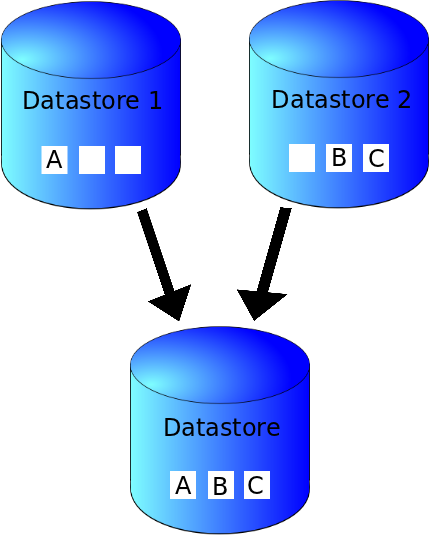
\includegraphics[scale=0.5]{project/images/data-sync}
  \caption{\textbf{IMAGE CAPTION}}
\end{figure}

\begin{lstlisting}
  PASTE YOUR CODE HERE
\end{lstlisting}
\newpage

 % adds the Project Design
\chapter{Screenshots of Project}
\section{SECTION NAME}
\vspace{2cm}
\begin{figure}[H]
  \centering
    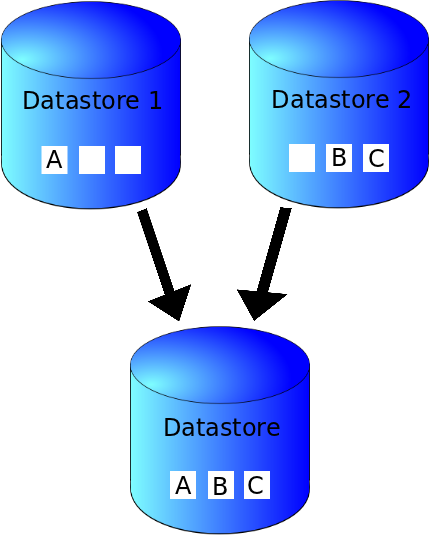
\includegraphics[height= 11cm, width=17cm]{project/images/data-sync}
\end{figure}
\newpage
\begin{figure}[H]
  \centering
    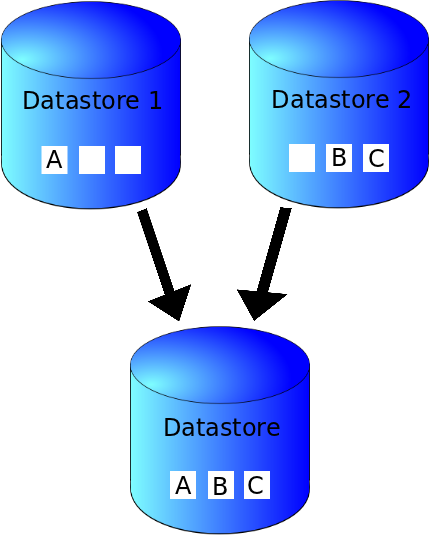
\includegraphics[height= 11cm, width=17cm]{project/images/data-sync}
\end{figure}
\vspace{1cm}
\begin{figure}[H]
  \centering
    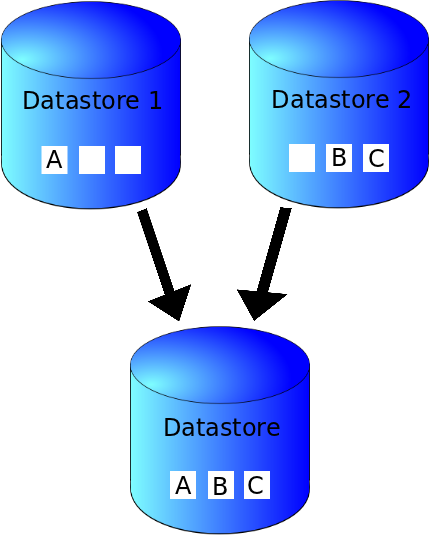
\includegraphics[height= 11cm, width=17cm]{project/images/data-sync}
\end{figure}
\section{CONCLUSION}

\paragraph{}
After this project, I have obtained many knowledge, first of all, is the usage of many design patterns and the way to implement them. Secondly, I have learned about the flexibility when apply the design pattern, there are many way to implement a design pattern. You should choose a way that suit the situation the best rather than just mimicking the sample code. Lastly, I have learned the way to use Latex more efficiently in making a report % adds the Scheduling and Planning page
%\addcontentsline{toc}{chapter}{References}
\begin{thebibliography}{99}
\bibitem{WRITE A SHORT-NAME WITHOUT SPACE} \emph{NAME OF IEEE PAPER}; NAME OF AUTHORS
\bibitem{WRITE A SHORT-NAME WITHOUT SPACE} \url{http://EXAMPLE.com}
\end{thebibliography} % adds the References page

\end{document}